\begin{frame}{Story-Explorer Idee}
  \begin{itemize}
    \item Open Data der Stadt Wien soll auch f\"{u}r Menschen ohne technischen Hintergrund verst\"{a}ndlich sein.
    \item Statt isolierter Datens\"{a}tze zeigt die App kurze, leicht lesbare Datenstorys.
    \item Der Ablauf bleibt bewusst einfach: Thema w\"{a}hlen $\rightarrow$ Datensatz w\"{a}hlen $\rightarrow$ Story verstehen.
  \end{itemize}
\end{frame}
%
\begin{frame}{Prototyp - Startseite}
  \centering
  \begin{tikzpicture}
    \node[anchor=center] (img) {%
      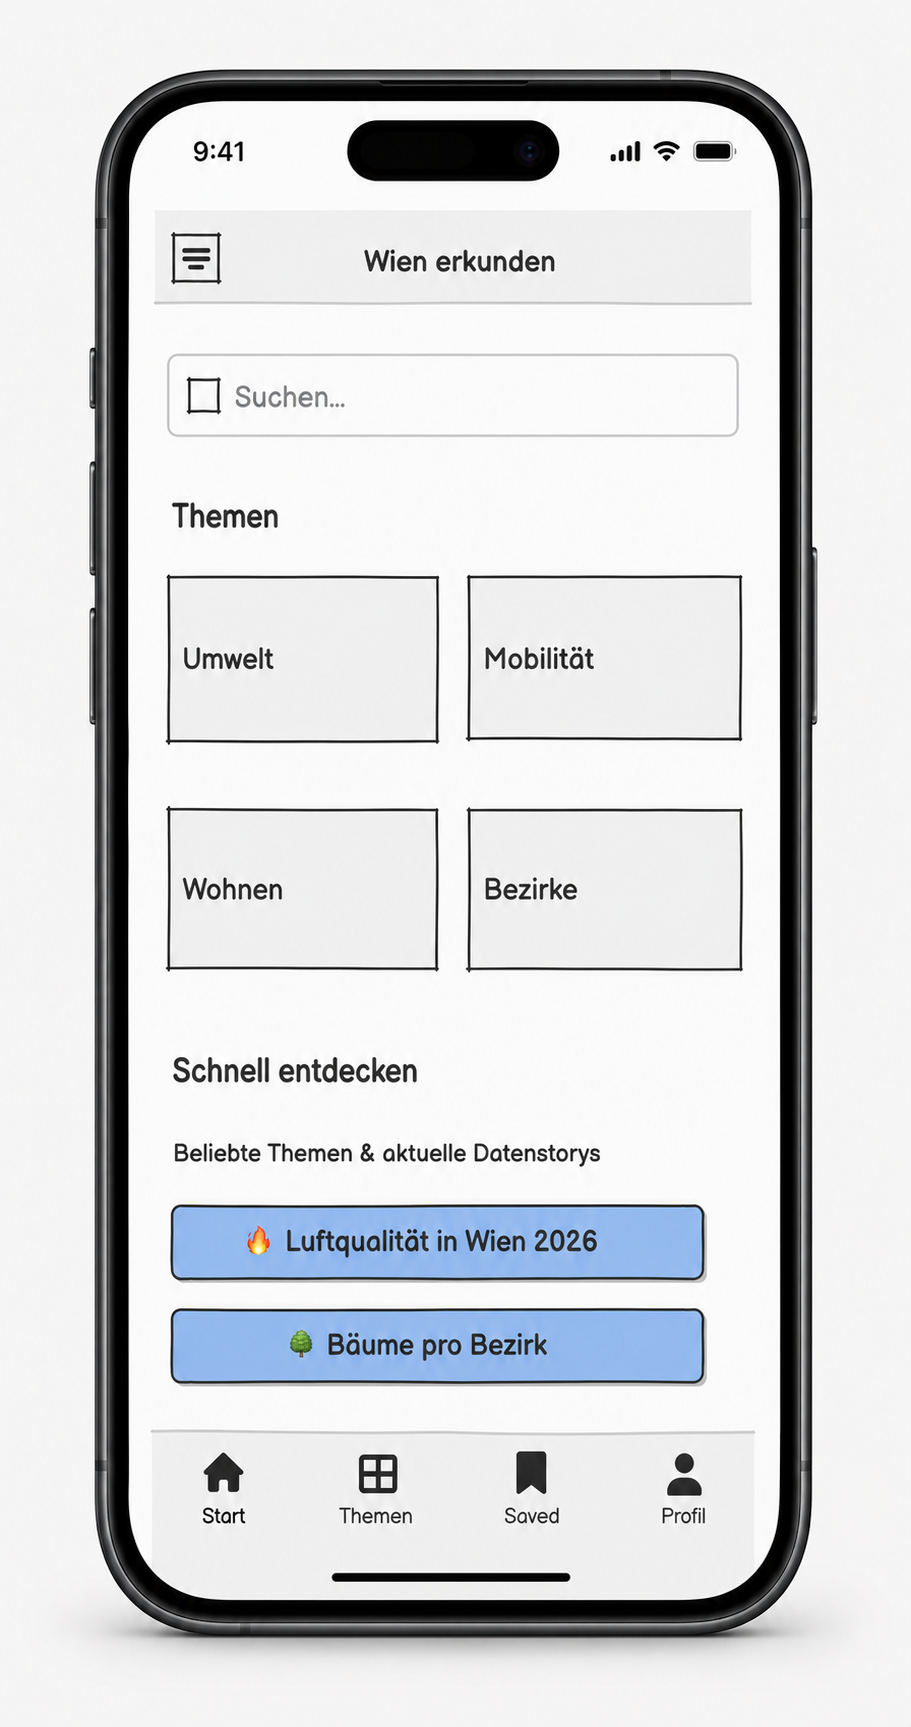
\includegraphics[width=0.90\textwidth,height=0.80\textheight,keepaspectratio]{images/Prototype_1.png}%
    };
    \draw[-{Stealth[scale=1.5]}, orange, line width=2pt]
      ($(img.center)+(-2.5cm, 1.5cm)$) -- ($(img.center)+(-1.0cm, 0.5cm)$)
      node[above left, orange, font=\small\bfseries] at ($(img.center)+(-2.5cm, 1.5cm)$) {Umwelt};
  \end{tikzpicture}
\end{frame}
%
\begin{frame}{Prototyp - Theme\"{u}bersicht}
  \centering
  \begin{tikzpicture}
    \node[anchor=center] (img) {%
      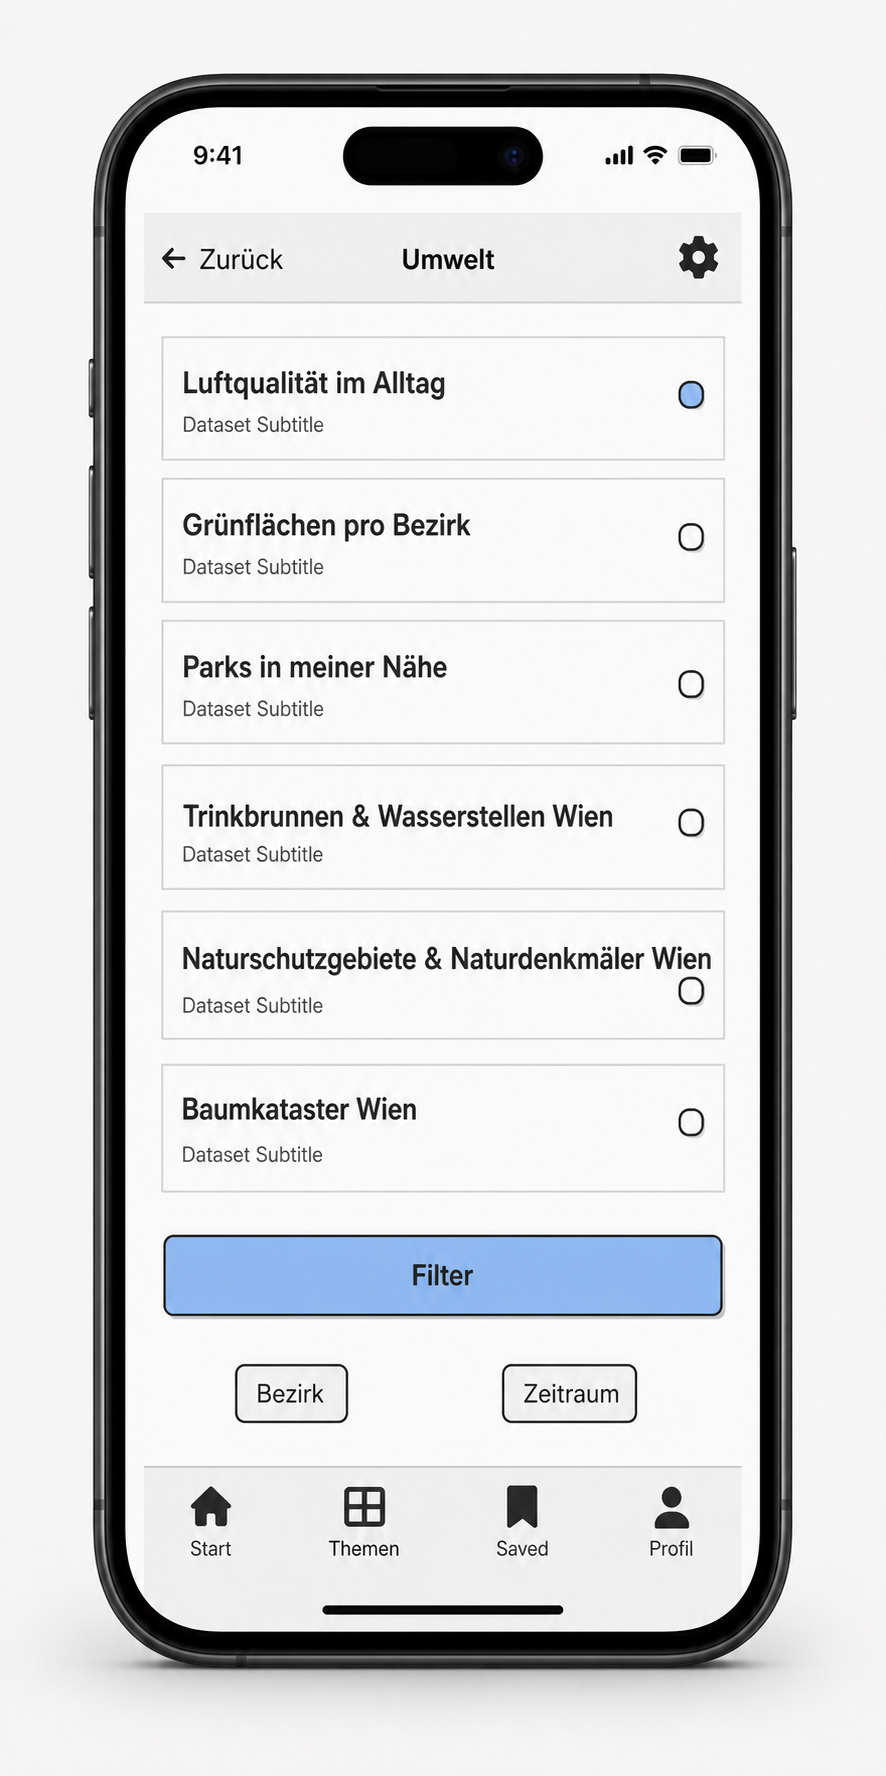
\includegraphics[width=0.90\textwidth,height=0.80\textheight,keepaspectratio]{images/Prototype_2.png}%
    };
    \draw[-{Stealth[scale=1.5]}, orange, line width=2pt]
      ($(img.center)+(-3.2cm, 2.0cm)$) -- ($(img.center)+(-1.3cm, 2.0cm)$);
  \end{tikzpicture}
\end{frame}
%
\begin{frame}{Prototyp - Story-Ansicht}
  \centering
  \begin{tikzpicture}
    \node[anchor=center] (img) {%
      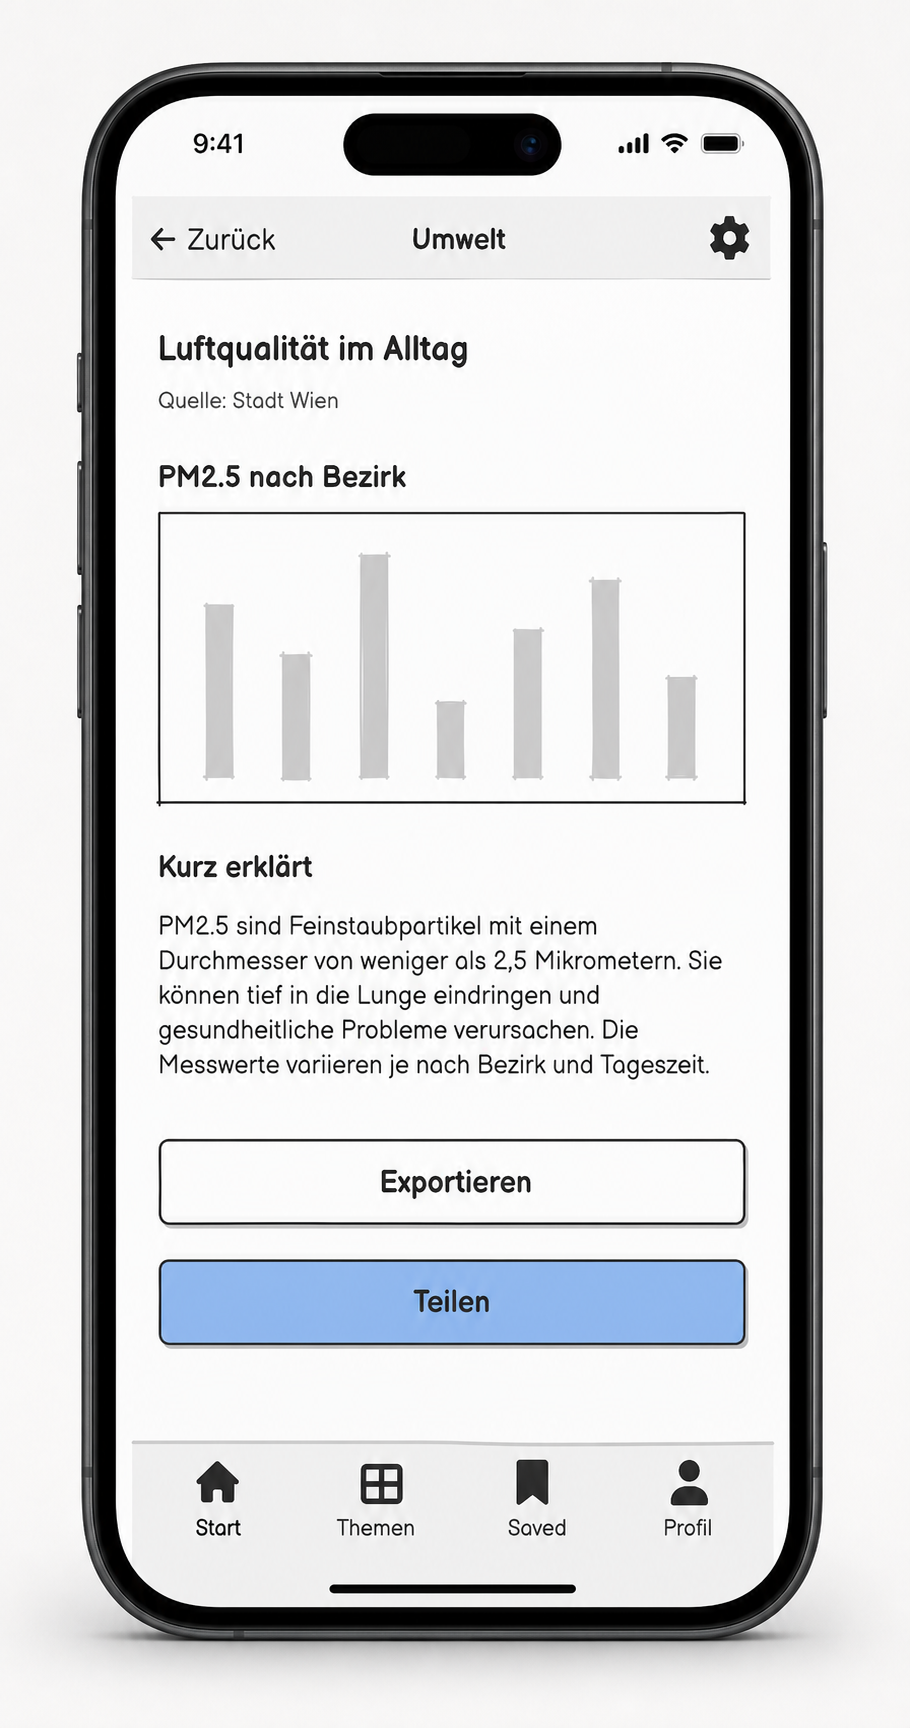
\includegraphics[width=0.90\textwidth,height=0.80\textheight,keepaspectratio]{images/Prototype_3.png}%
    };
  \end{tikzpicture}
\end{frame}
%
\begin{frame}{Anpassung an Personas}
  \begin{itemize}
    \item{Benjamin:} Filter nach Bezirk und Zeitraum f\"{u}r gezielte Suche.
    \item{Leah:} Teilen und Exportieren sind direkt sichtbar.
    \item{Ralph:} Klare Quellenangaben schaffen Transparenz und Vertrauen.
    \item{Luca:} Einfache Einstiege und kurze Erkl\"{a}rungen senken die H\"{u}rde.
  \end{itemize}
\end{frame}
%
\begin{frame}{Evaluierung}
  \begin{block}{Feedback}
    \vspace{0.5em}
    Der klare Ablauf und der ,,Kurz erkl\"{a}rt``-Abschnitt wurde besonders gut gefallen.
  \end{block}

  \vspace{0.5em}
  \textbf{Bevorzugte Kombination:} Story Explorer + Personalisierung von Wien in Zahlen

  \vspace{0.5em}
  \textbf{Verbesserungswunsch:}
  \begin{itemize}
    \item Datens\"{a}tze werden antippbar sein.
  \end{itemize}
\end{frame}
